\documentclass[10pt]{article}
\usepackage{../../local}


\newcommand{\classcode}{Physics 89}
\newcommand{\classname}{Mathematical Methods in Physics}
\renewcommand{\maketitle}{%
\hrule height4pt
\large{Yutong (Eric) Du \hfill \classcode}
\newline
\large{HW 01} \Large{\hfill \classname \hfill} \large{\today}
\hrule height4pt \vskip .7em
\normalsize
}
\linespread{1.1}
\newcommand{\Arg}{\mathrm{Arg}}
\begin{document}
	\maketitle
	\section*{Problem 1.1}

	In lecture we saw how to use Taylor approximations to find the potential along the axis of an \textbf{
	\textit{electric dipole}}. In this problem we will expand on this analysis to study \textbf{\textit{electric
multipoles}}. Recall that the potential due to a \textit{single} point charge $q$ a distance $r$ away is 
given by 
\[
V = \frac{kq}{r}
\] 
	Consider an electric dipole consisting of a positive charge $+q$ on the $x$-axis at $x = d/2$ and an equal
	and opposite negative charge $-q$ on the $x$-axis at $x = d/2$ as shown.

	\begin{enumerate}[label=\alph*)]
		\item Find the lowest-order approximation to the potential at a general point $(x, y) = (r \cos \theta, 
			r \sin \theta)$ when $r \gg d$. 

			\begin{solution}
				Let us define two quantities $r_+$ and $r_-$ defined as shown in the diagram below
				
				\begin{center}
					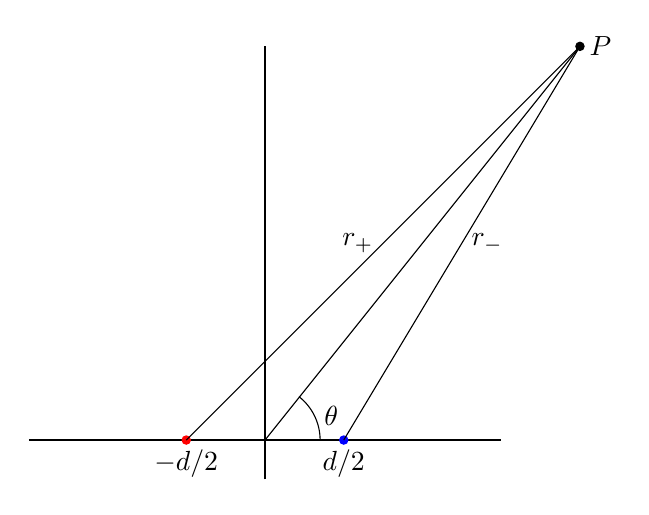
\begin{tikzpicture}
						\draw[thick]  (-3, 0) -- (3, 0);
						\draw (1, 0) node[below] {$d/2$};
						\filldraw[red] (-1, 0) circle (1.5pt);
						\filldraw[blue] (1, 0) circle (1.5pt);
						\draw (-1, 0) node[below] {$-d / 2$};
						\draw[thick] (0, -0.5) -- (0, 5);
						\draw(0, 0) -- (4, 5) node[above, right] {$P$};
						\filldraw (4, 5) circle (1.5pt); 
						\draw (0.7, 0) arc(0:52:0.7) node[midway, above, right] {$\theta$}; 
						\draw (1, 0) -- (4, 5) node[midway, right] {$r_-$};
						\draw (-1, 0) -- (4, 5) node[midway, above, left] {$r_+$};
					\end{tikzpicture}
				\end{center}

				From the diagram, we can use cosine law:
				\begin{align*}
					r_-^2 &= \left( \frac{d}{2} \right)^2 + r^2 - 2r \frac{d}{2}\cos \theta = 
					\left( \frac{d}{2} \right)^2 + r^2 - r d \cos \theta \\
					r_+^2 &= \left( \frac{d}{2} \right)^2 + r^2 - 2r \frac{d}{2}\cos(\pi - \theta) =
					\left( \frac{d}{2} \right)^2 + r^2 + r d \cos \theta 
				\end{align*}		
				The first order approximation is sufficient here so we can neglect the $(\frac{d}{2})^2$ term, 
				which then allows us to factor out $r^2$ from both expressions:
				\begin{align*}
					r_+^2 &= r^2 + r d \cos \theta  = r^2\left(1 + \frac{d}{r}\cos \theta\right) \implies 
					r_+ = r\left( 1 + \frac{d}{r}\cos \theta \right)^{1/2} \\
					r_-^2 &= r^2 - r d \cos \theta = r^2\left( 1 - \frac{d}{r}\cos \theta \right) \implies
					r_- = r\left( 1 - \frac{d}{r}\cos \theta \right)^{1/2}
				\end{align*}
				Now let's go back to the potential and add up the contributions due to the positive and negative
				charges:
				\begin{align*}
					V = \frac{kq}{r_-} - \frac{kq}{r_+} &= kq\left( \frac{1}{r_-} - \frac{1}{r_+} \right) 
				\end{align*}
				Now we can substitute what we have for $r_+$ and $r_-$, while letting $\epsilon = \frac{d}{r}$:
				\begin{align*}
					V &= kq\left[\frac{1}{r(1 - \epsilon \cos \theta)^{1 / 2}} - \frac{1}{r(1 + \epsilon 
					\cos \theta)^{1/2}}\right] \\
					  &= \frac{kq}{r}\left[(1 - \epsilon \cos \theta)^{- 1 / 2} - (1 + \epsilon \cos \theta)^{-
					  1/2}\right]\\
					  &= \frac{kq}{r}\left[1 + \frac{1}{2}\epsilon \cos \theta - (1 - \frac{1}{2}\epsilon \cos
					  \theta)\right]\\
					  &= \frac{kq}{r}(\epsilon \cos \theta) \\
					  &= \frac{kqd \cos \theta}{r^2}
				\end{align*}
			\end{solution}
	\end{enumerate}

	Next consider a \textbf{\textit{linear electric quadrupole}}, with a point charge $+2q$ at the origin, 
	a point charge $-q$ at $x = +d$ and a point charge $-q$ at $x = -d$. Consider a point $P$ at position $x$
	on the $x$-axis and a good distance to the right of the quadrupole so $x \gg d$. 

	\begin{enumerate}[label=\alph*), resume]
		\item Find the lowest-order approximation to the potential at point $P$ when $x \gg d$. 

			\begin{solution}
				First we write the potential out fully:
				\[
				V = k\left( -\frac{q}{x - d} + \frac{2q}{x} - \frac{q}{x + d} \right) = kq\left( 
				\frac{2}{x} - \frac{1}{x - d} - \frac{1}{x+d}\right) 
				\] 
				Then since $\frac{d}{x} \ll 1$, then let $\epsilon = \frac{d}{x} \implies d = \epsilon x$. 
				Substituting this in: 
				\[
				V = \frac{kq}{x}\left( 2 - \frac{1}{1 - \epsilon} - \frac{1}{1 + \epsilon } \right) 
				\] 
				The taylor expansions of the two fractions are as follows:
				\begin{align*}
					\frac{1}{1 + \epsilon} &= (1 + \epsilon)^{-1} = 1 - \epsilon + \epsilon^2 + O(\epsilon^3)\\
					\frac{1}{1 - \epsilon} &= (1 + (-\epsilon))^{-1} = 1 + \epsilon + \epsilon^2 + O(\epsilon^3)
				\end{align*}
				we only take these to second order since that's the first nonzero term. Now combining 
				everything together:
				\[
				V \approx \frac{kq}{x}(2 - (1 + \epsilon + \epsilon^2) - (1 - \epsilon + \epsilon^2)) =
				\frac{kq}{x}(-2\epsilon^2) = -\frac{2kqd^2}{x^3}
				\] 

			\end{solution}
	\end{enumerate}
	
	\pagebreak
	\section*{Problem 1.2}

	In class we presented the Taylor expansions for $\sin(x)$ and $\cos(x)$ about the point $x = 0$,
	\[
		\sin(x) = \sum_{n = 0}^\infty \frac{(-1)^n x^{2n + 1}}{(2n + 1)!}, \phantom{aaaa} \cos(x) = 
		\sum_{n = 0}^\infty \frac{(-1)^n x^{2n}}{(2n)!}
	\] 

	\begin{enumerate}[label=\alph*)]
		\item Let $f(x) = \sin(x)$ and explicitly carry out the Taylor expansion about the point $x = 0$. Show
			that your answer reproduces the formula for $\sin(x)$ shown above.

			\begin{solution}
				Taking the derivatives, we get the following:
				\begin{align*}
					f(0) &=  0 \\
					f'(0) &=  \cos(0) = 1 \\
					f''(0) &= -\sin(0) = 0 \\
					f'''(0) &= -\cos(0) = -1 \\
							&\vdots
				\end{align*}
				The nonzero derivatives occur whenever we have a $\cos(0)$ term. This pattern occurs at every 
				other term, since taking the derivative of $\sin(x)$ gives us $\cos(x)$ (giving us a nonzero
				term), and taking the derivative of $\cos(x)$ gives us $\sin(x)$, giving us a zero. Taking the 
				derivative again returns us to $\cos(x)$, which is nonzero again hence there is a pattern that 
				every other term is nonzero. Therefore, we get:
				\[
				\sin(x) \approx x - \frac{x^3}{3!} + \frac{x^5}{5!} - \frac{x^7}{7!} + O(x^9)
				\] 
				This matches the series expansion, since for $n = 0$ we would get $x$, then $n = 1$ gives us 
				the $-x^3 / 3!$ term, and so on. In the expansion, we are neglecting the indices that give us 
				zero by using $2n + 1$ as the index in the summation rather than just $n$, meaning that 
				our index ``step size" is 2. In other words, we are allowed to ``skip over'' the even indices
				because they are all zero. 
			\end{solution}
		\item Graph $\sin(x)$, and the first, third, and fifth order Taylor series approximation to $\sin(x)$ 
			in the range $-3\pi/2 \le x \le 3\pi/2$. 

			\begin{solution}
				Below I've plotted the sine curve over the $x \in [-3\pi/2, 3 \pi /2]$. The blue curve is the full sine 
				curve, and the other colors are the approximations. 

				\begin{center}
					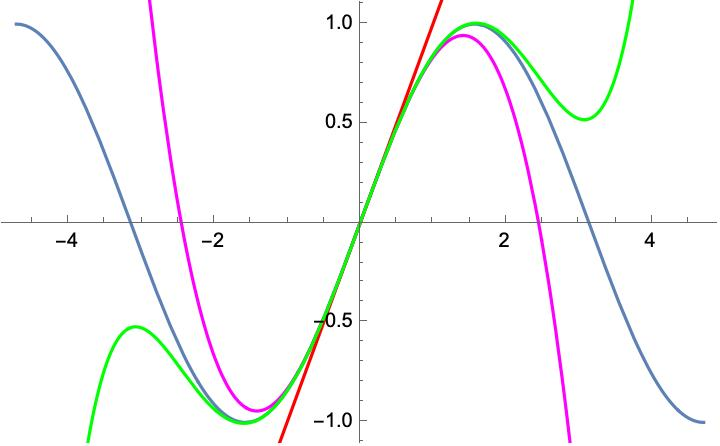
\includegraphics[scale=0.5]{sine.jpeg}
				\end{center}
			\end{solution}
	\end{enumerate}
	Some functions can't be Taylor expanded about certain points. For example, if we try to Taylor expand
	$1/x$ about the point $x = 0$ we would fail since $1/x = \infty$! In such cases, it may be possible to expand
	the function using both positive and \textit{negative} powers of $x$. For example, we can express the 
	function $\sin(x)/x^2$ as,
	\[
		\frac{\sin x}{x^2} \approx \frac{x - x^3/3! + x^5/5! + \mathcal O(x^7)}{x^2} = \frac{1}{x} -
		\frac{x^2}{3!} + \frac{x^3}{5!} + \mathcal O(x^5)
	\] 
	Such a series is a generalization of the Taylor series called the \textbf{\textit{Laurent Series}}, which 
	is an enormously useful tool in complex analysis.
	\begin{enumerate}[label=\alph*),resume ]
		\item Use the two series for $\sin(x)$ and $\cos(x)$ to find the Laurent series/small-angle approximation
			for $\cot(x)$ to the lowest two non-zero terms. Check your approximation by finding $\cot(0.1)$ and
			comparing with your approximation. How about for $\cot(1)$? $\cot(\pi/2)$?

			\begin{solution}
				We know that $\cot(x) = \frac{\cos(x)}{\sin(x)}$, so therefore we can take the first two 
				terms of the Taylor expansion for $\sin(x)$ and $\cos(x)$:
				\begin{align*}
					\cot(x) &= \left(1 - \frac{x^2}{2!}\right)\left(x - \frac{x^3}{3!}\right)^{-1} \\
							&= \left( 1 - \frac{x^2}{2!} \right) \cdot \frac{1}{x} \cdot 
							\left( 1 - \frac{x^2}{3!} \right)^{-1}
				\end{align*}
				Now we can use the binomial expansion to simplify the term with the negative exponent: 
				\[
					(1 - x)^{n} = 1 - nx + O(x^2)
				\] 
				Doing so, we get:
				\begin{align*}
					\cot(x) &=  \left( 1 - \frac{x^2}{2!} \right) \cdot \frac{1}{x} \cdot 
					\left(1 - \frac{x^2}{3!}\right) \\
							&= \frac{1}{x}\left[1 - \frac{x^2}{3!} - \frac{x^2}{2!} - \frac{x^4}{2!3!}\right]
				\end{align*}
				Keeping the first two terms only, we get:
				\[
				\cot(x) \approx \frac{1}{x} - \frac{x}{3}
				\] 
				Using Mathematica, we find that $\cot(0.1) = 9.96664$, and our Taylor approximation gives
				9.96667, which indicates that it's a very good approximation. Then, with the other values, we 
				get:

				\begin{center}
					\begin{tabular}{c|c|c}
						Input         & Exact     & Taylor Approximation \\ \hline
						$\cot(1)$     & 0.6420... & 0.6666...            \\ \hline
						$\cot(\pi/2)$ & 0         & 0.1130              
					\end{tabular}
				\end{center}
				We can see that since we centered our taylor approximations around $x = 0$, that our 
				approximations for $\cot(x)$ around $x = 0$ is quite good (difference of 0.00003), but the
				approximation starts to fail 
				once we get to $x= \frac{\pi}{2}$, where the difference jumps to over 0.1.
			\end{solution}
		\item Use the Taylor series for $e^x$, $\sin(x)$ and $\cos(x)$ to show \textbf{\textit{Euler's formula}}
			\[
				e^{i \theta} = \cos(\theta) + i \sin(\theta)
			\] 

			\begin{solution}
				We have the series of $\sin(x)$ from part (a), but I'll repeat it here:
				\[
				\sin(x) = x - \frac{x^3}{3!} + \frac{x^5}{5!} - \frac{x^7}{7!} + O(x^9)
				\] 
				The expansion for $\cos(x)$ is:
				\[
				\cos(x) = 1 - \frac{x^2}{2!} + \frac{x^4}{4!} - \frac{x^6}{6!} + O(x^8)
				\] 
				The expansion for $e^x$ is:
				\[
				e^x = 1 + x + \frac{x^2}{2} + \frac{x^3}{3!} + \frac{x^4}{4!} + O(x^5)
				\] 
				then plugging in $x = i \theta$ into the last series, we have:
				\[
					e^{i \theta} = 1 + i \theta - \frac{\theta^2}{2}-\frac{i\theta^3}{3!}=\underbrace{\left( 1 -
					\frac{\theta^2}{2!} + \frac{\theta^4}{4!}  + \dots \right)}_{= \cos(\theta)} +
					i \underbrace{\left( \theta
			- \frac{\theta^3}{3!} + \frac{\theta^5}{5!} + \dots \right)}_{= \sin(\theta)}  = \cos(\theta) + i
			\sin \theta
				\] 
			\end{solution}
	\end{enumerate}
	\pagebreak

	\section*{Problem 1.3}
	\begin{enumerate}[label=\alph*)]
		\item Let $z_1 = x_1 + iy_1 = r_1e^{i \theta_1}$ and $z_2 = x_2 + iy_2 = r_2e^{i \theta_2}$. Find the 
			real part and imaginary part of the product $z_1z_2$ and the quotient $z_1/z_2$ in terms of the 
			Cartesian components $x_1, x_2, y_1$ and $y_2$. Then find the real and imaginary part of the product
			$z_1z_2$ and the quotient $z_1/z_2$ in terms of the polar components $r_1, r_2, \theta_1$ and 
			$\theta_2$.

			\begin{solution}
				The product is:
				\[z_1z_2 = (x_1 + iy_1)(x_2 + iy_2) = x_1x_2 - y_1y_2 + i(x_1y_2 + y_1x_2)\]
				so the real part is $\Re(z_1z_2) = x_1x_2 - y_1y_2$, and the complex part is
				$\Im(z_1z_2) = x_1y_2 +y_1x_2$. The quotient is:
				\[
				\frac{z_1}{z_2} = \frac{x_1 + iy_1}{x_2 + iy_2} = \frac{(x_1 + iy_1)(x_2 - iy_2)}{x_2^2 + y_2^2}
				= \frac{x_1x_2 + y_1y_2 -i(x_1y_2 + x_2y_1)}{x_2^2 + y_2^2}
				\] 
				Here, the real part is: 
				\[
				\Re\left( \frac{z_1}{z_2} \right) =  \frac{x_1x_2 + y_1y_2}{x_2^2 + y_2^2}
				\] 
				and the imaginary part is:
				\[
				\Im\left( \frac{z_1}{z_2} \right) =	-\frac{x_1y_2 + x_2y_1}{x_2^2 + y_2^2}
				\] 
				With the other representation, the product $z_1z_2 = r_1r_2 e^{i(\theta_1 + \theta_2)}$. We
				then have to break up the complex exponential into its real and imaginary part (using 
				$e^{i \theta} = \cos \theta + i \sin \theta$), so we get:
				\[
					\Re(z_1z_2) = r_1r_2\cos (\theta_1 + \theta_2) \phantom{aaaaaa} \Im(z_1z_2) = r_1r_2
					\sin(\theta_1 + \theta_2)
				\] 
				For the quotient, we have:
				\[
					\frac{z_1}{z_2} = \frac{r_1e^{i \theta_1}}{r_2e^{i \theta_2}} = \frac{r_1}{r_2}e^{i (\theta_1 - \theta_2)}
				\] 
				Again, splitting this up using the identity $e^{i \theta} = \cos \theta + i \sin \theta$, we 
				get:
				\[
					\Re\left(\frac{z_1}{z_2}\right) = \frac{r_1}{r_2}\cos(\theta_1 - \theta_2) \phantom{aaaa}
					\Im\left(\frac{z_1}{z_2}\right) = \frac{r_1}{r_2}\sin(\theta_1 - \theta_2)
				\] 
			\end{solution}
		\item Let $z = x+ iy = re^{i \theta}$. Find $|z|^2$ and $z^2$ first in terms of $x$ and $y$ and then 
			in terms of $r$ and $\theta$. Under what circumstances does $|z|^2 = z^2$?

			\begin{solution}
				The modulus square $|z|^2 = x^2 + y^2 = r^2$, whereas the square $z^2 = x^2 + 2ixy - y^2 = r^2
				e^{2i\theta}$. Equality only occurs when the imaginary part disappears, so when $y = 0$. This 
				also corresponds to $\theta = 0, \pi, 2\pi, \dots$ (every integer multiple of $\pi$).
			\end{solution}
		\item Use Euler's formula on both sides of $e^{i(\alpha + \beta)} = e^{i \alpha}e^{i \beta}$ to derive
			the formulas for $\cos(\alpha + \beta)$ and $\sin(\alpha + \beta)$

			\begin{solution}
				On the left hand side we have
				\[
					e^{i(\alpha + \beta)} = \cos(\alpha + \beta) + i \sin(\alpha + \beta)
				\] 
				and on the right hand side we have to do some multiplication: 
				\begin{align*}
					e^{i \alpha} e^{i \beta} &= (\cos \alpha + i \sin \alpha)(\cos \beta + i \sin \beta) \\
					&= \cos \alpha \cos \beta - \sin \alpha \sin \beta + i(\sin \alpha \cos \beta + \cos \alpha
					\sin \beta)
				\end{align*}
				So comparing the real and imaginary parts, we get the identities:
				\begin{align*}
					\cos(\alpha + \beta) &= \cos \alpha \cos \beta - \sin \alpha \sin \beta\\
					\sin(\alpha + \beta) &= \sin \alpha \cos \beta + \cos \alpha \sin \beta 
				\end{align*}
			\end{solution}

	\end{enumerate}
	Let $z_1 = r_1e^{i \theta_1}$ and $z_2 = r_2 e^{i \theta_2}$
	\begin{enumerate}[label=\alph*),resume ]
		\item Show that $|z_1 + z_2| = \sqrt{r_1^2 + r_2^2 + 2r_1r_2\cos(\theta_1 - \theta_2)}$  

			\begin{solution}
				We can do this by finding the norm-squared:
				\begin{align*}
					|z_1 + z_2|^2 &= |r_1e^{i \theta_1} + r_2e^{i \theta_2}|^2\\
								  &= (r_1e^{i \theta_1} + r_2e^{i \theta_2})(r_1e^{-i\theta_1} + r_2e^{-i 
								  \theta_2})\\
								  &= r_1^2 + r_2^2 + r_1r_2 e^{i(\theta_1 - \theta_2)} + r_1r_2 e^{i(\theta_2
								  - \theta_1)}\\
								  &= r_1^2 + r_2^2 + r_1r_2\left( e^{i (\theta_1 - \theta_2)} + e^{-i(
								  \theta_1 - \theta_2)}\right)
				\end{align*}	
				Now we use the identity:
				\[
					\cos(x) = \frac{e^{ix} + e^{-ix}}{2}
				\]
				with $x = \theta_1 - \theta_2$ in this case, so therefore:
				\[
				|z_1 + z_2|^2 = r_1^2 + r_2^2 + 2r_1r_2\cos(\theta_1 - \theta_2)
				\] 
				taking the square root:
				\[
				|z_1 + z_2| = \sqrt{r_1^2 + r_2^2 + 2r_1r_2\cos(\theta_1 - \theta_2)} 
				\] 
			\end{solution}
		\item (Extra) Use the result from part (d) to show the \textbf{\textit{triangle inequality}} $|z_1 + z_2|
			\le |z_1| + |z_2|$. Under what conditions is the inequality \textbf{\textit{saturated}}.

			\begin{solution}
				We expand $|z_1| + |z_2| = r_1 + r_2 = \sqrt{(r_1 + r_2)^2} = \sqrt{r_1^2 + r_2^2 + 2r_1r_2}$.
				Note that since $-1 \le \cos(\theta_1 - \theta_2) \le 1$, the quantity $2r_1r_2 \ge 
				2r_1r_2\cos(\theta_1 - \theta_2)$, and so overall the triangle inequality holds. Equality is 
				reached when $\theta_1 - \theta_2 = 0, 2\pi, \dots$ or in general: $\theta_1 - \theta_2 = 2n \pi$
				where $n = 1, 2, \dots$.
			\end{solution}
		\item Show \textbf{\textit{De Moivre's formula}}, $(\cos \theta + i \sin \theta)^n = \cos(n \theta) + i
			\sin (n\theta)$. 

			\begin{solution}
				On the left hand side, we can rewrite $\cos \theta + i \sin \theta = e^{i \theta}$, so therefore
				\[
					(e^{i \theta})^n = e^{in \theta} = \cos(n \theta) + i \sin(n \theta)
				\] 
				as desired. 
			\end{solution}
	\end{enumerate}
	Let $n \in \mathbb N$ (that is, $n$ is a positive whole number). The \textbf{\textit{n-th root}} of a complex
	number $z$ is $z^{1/n}$. When dealing with roots we have to be careful when the  $n$-th root function is 
	\textbf{\textit{multi-valued}}. In particular, there are $n$ different possible values of $w$ such that $w^n
	 = z$, all of which could properly be considered $n$-th roots of $z$. Let's explore this. 
	 \begin{enumerate}[label=\alph*),resume]
	 	\item Consider the three different cube-roots of $z = i$ (which, using Euler's formula, we can also 
			write as $e^{i \pi/2}$. Show that $w = e^{i \pi/6}, e^{5i \pi/6}$, and $e^{3i\pi/2}$ all cube to 
			$z = i$. Plot these roots on the complex plane and demonstrate graphically how $e^{5 i \pi/6}$ cubes
			to $i$. 

			\begin{solution}
				Let $w_1, w_2, w_3$ be the solutions. Then, we have $w_1^3 = e^{3i \pi / 6} = e^{i \pi /2} = i$,
				$w_2^3 = e^{15 i \pi / 6} = e^{5 i \pi /2} = e^{2 i \pi + i \pi / 2} = e^{i \pi /2} =i$ and 
				finally $w_3^3 = e^{9 i \pi /2} = e^{8 i \pi + i \pi /2} = e^{i \pi /2} = i$. Graphically
				speaking, when we cube $e^{5i\pi / 6}$ we are rotating the vector $e^{5 i \pi / 6}$ by the 
				angle $5 \pi /6$ two times, which comes out to a total angle of $15 \pi /6$, which is the same
				as rotating by $\pi / 2$, as shown below:
				\begin{center}
					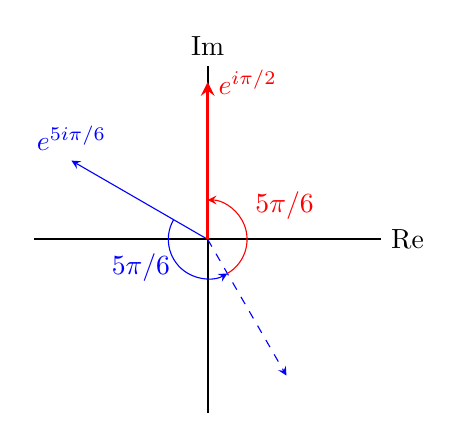
\begin{tikzpicture}
						\draw[thick] (-2.2, 0) -- (2.2, 0) node[right] {Re};
						\draw[thick] (0, -2.2) -- (0, 2.2) node[above] {Im};
						\draw[-stealth, blue](0, 0) -- (-1.73, 1) node[above] {$e^{5 i \pi / 6}$};
						\draw[-stealth, dashed, blue] (0, 0) -- (1, -1.73);
						\draw[-stealth, red, very thick] (0, 0) -- (0, 2) node[right] {$e^{i\pi / 2}$};
						\draw[-stealth, blue] (-0.433, 0.25) arc (150:300:0.5) node[midway, left] {$5 \pi / 6$};
						\draw[-stealth, red] (0.25, -0.433) arc (300:450:0.5) node[midway, above right] {$ 5 \pi / 6$};
					\end{tikzpicture}
				\end{center}
				Here, we see that the solid blue arrow represents the initial vector $e^{5 i \pi /6}$, and when 
				we multiply it by $e^{5 i \pi /6}$ once, we get the dashed blue line, and when we multiply 
				it again we get the red vector, which is also represented by $e^{i \pi /2}$. 

				The problem also asks for each of the roots to be plotted, so here they are:

				\begin{center}
					\begin{tikzpicture}
						\draw[thick] (-2.2, 0) -- (2.2, 0) node[right] {Re};
						\draw[thick] (0, -2.2) -- (0, 2.2) node[above] {Im};
						\draw[-stealth, blue](0, 0) -- (-1.73, 1) node[above] {$e^{5 i \pi / 6}$};
						\draw[-stealth, blue](0, 0) -- (1.73, 1) node[right] {$e^{i \pi /6}$};
						\draw[-stealth, blue, very thick](0, 0) -- (0, -2) node[right] {$e^{3 i \pi /2}$};
					\end{tikzpicture}
				\end{center}
			\end{solution}
		\item (Extra) Show that the $n$ distinct values of the $n$-th root of $z = re^{i \theta}$ are $w_k = 
			r^{1/n}e^{i(\theta + 2\pi k)/n}$, with $k = 0, \cdots, n - 1$. As a check, test that your formula 
			implies that if $w$ is a square root of $z$ then so is $-w$.

			\begin{solution}
				Taking any of the roots $w_k$ to the $n$-th power, we get:
				\[
					w_k^n = re^{i(\theta + 2\pi k)} = re^{i \theta} e^{2 \pi i k} 	
				\] 
				the term $e^{2 \pi i k}$ represents an integer multiple of $2\pi$ revolutions, which is 
				the same thing as multiplying by 1, and thus we've proven equality. We can also see this 
				explicitly by remembering the identity $e^{2 \pi i} = 1$, so therefore 
				\[
					e^{2 \pi i k} = (e^{2 \pi i})^k = 1^k = 1
				\] 
				which is another way to show that $re^{i \theta} e^{2 \pi i k} = re^{i \theta}$.
			\end{solution}
	 \end{enumerate}
	 The multi-valued nature of the $n$-th root ultimately comes from the multi-valued nature of the logarithm. 
	 Recall that 
	 \[
	  \ln z = \ln|z| + i \Arg(z) + 2 \pi ik
	 \] 
	 where $\Arg(z)$ = $\tan^{-1}(y/x)$ is the \textbf{\textit{principle value}} of the argument, so $-\pi < 
	 \Arg(z) \le \pi$, and $k \in \mathbb Z$ is the \textbf{\textit{branch index}}. Before solving part (i), be
	 sure to convince yourself that the exponentian of the right-hand side of Eq.1 does indeed produce $z = |z|
	 e^{i \Arg(z)}$ for any integer $k$. 
	 \begin{enumerate}[label=\alph*), resume]
	 	\item Use Eq.1 to solve the formula $w^n = z$ for $w$ by first taking the logarithm of both sides, 
			solving for $\ln w$, and then exponentiating. You should get back your formula from part (h)!

			\begin{solution}
				We follow the problem and take the logarithm of both sides and solving for $\ln w$:
				\begin{align*}
					n \ln w &=  \ln z \\
					\ln w &= \frac{1}{n} \ln z
				\end{align*}
				Now we then exponentiate:
				\begin{align*}
					w &= e^{\frac{1}{n}\ln z}\\
					  &=  e^{\frac{1}{n}(\ln |z| + i \Arg(z) + 2 \pi i k)} \\
					  &= |z|^{1/n} e^{(i \Arg(z) + 2 \pi i k) / n} \\
					  &= r^{1 / n}e^{i(\theta + 2 \pi k) / n}
				\end{align*}
				as desired. 
			\end{solution}
	 \end{enumerate}
	 \pagebreak
	 \section*{Problem 1.4}

	 Consider a mass $m$ at the end of an ideal spring with spring constant $k$ (so the spring force is 
	 $F_{\text{spring}} = -kx$). In introductory physics when studying this system, you find that the mass
	 undergoes \textit{oscillatory} motion with angular frequency $\omega_0 = \sqrt{k/m}$. Now let's make 
	 the physical system a little more physically accurate by adding in the effects of \textbf{\textit{damping}},
	 a type of friction force (it removes mechanical energy from the system). The damping force is proportional
	 to the velocity, $F_{\text{damping}} = -2 m \gamma v$, where $\gamma \ge 0$ is the 
	 \textbf{\textit{damping coefficient}}. Therefore, 
	 \[
	 ma = -m\omega_0^2 x - 2m \gamma v
	 \] 
	 Our problem is ironically made less complicated by \textit{\textbf{complexifying}}. That is, we replace the
	 real position $x \in \mathbb R$ with a ``complex position'' $z \in \mathbb Z$ such that $\Re z \equiv x$. We
	 intuitively know or can guess what our damped sprign will behave like - it should oscillate with a 
	 decreasing amplitude. Therefore, we will make an \textbf{\textit{ansatz}} (a guess) at what the complex
	 position will look like, 
	 \[
		 z(t) = Ae^{i \Omega t} 
	 \] 
	 where $\Omega \in \mathbb C$ is a complex number with units of $[\Omega] = \mathrm s^{-1}$ and $A = A_0 
	 e^{i \phi_0}$ is some initial complex amplitude. We define $\omega \in \mathbb R$ and $\Gamma \in \mathbb R$
	 to be a real and imaginary parts of $\Omega$, 
	 \[
	 \Omega \equiv \omega + i \Gamma
	 \] 
	 \begin{enumerate}[label=\alph*)]
		 \item Express $z(t) = Ae^{i \Omega t}$ in polar form $r(t) e^{i \phi(t)}$, with $r(t)$ and $\phi(t)$ 
			 are \textit{real} functions expressed in terms of the real constants $\omega, \Gamma, A_0$ and 
			 $\phi_0$. Using your physical intuition (think about the actual motion of a damped oscillator
			 or think about energy), what condition must $\Gamma$ satisfy for our solution to be physically 
			 reasonable?

			 \begin{solution}
				 We have $z(t) = Ae^{i \Omega t}$, so we can write $\Omega = \omega + i \Gamma$:
				 \begin{align*}
					 z(t) &= Ae^{i \Omega t}\\
						  &= A_0e^{i \phi_0} e^{it(\omega + i \Gamma)} \\
						  &= A_0e^{i \phi_0}e^{i \omega t - \Gamma t} \\
						  &= A_0e^{-\Gamma t} e^{i(\phi_0 + \omega t)}
				 \end{align*}
				 And so we deduce that $r(t) = A_0e^{-\Gamma t}$ and $\phi(t) = \phi_0 + \omega t$. In order
				 for our solution to be physically reasonable, the motion it describes must either describe
				 a decaying amplitude or a constant one, since the damping coefficient is a friction force, and 
				 thus it cannot add energy to the system (it could however, do nothing, which would result 
				 in a constant amplitude). Therefore, the condition on $\Gamma$ is that 
				 $\Gamma \ge 0$. 
			 \end{solution}
	 \end{enumerate}
	 From the complex position $z$ we can define a complex velocity $\tilde v = \dv{z}{t}$ and a complex 
	 acceleration $\tilde a = \dv{\tilde v}{t}$, in whihc case Eq. 2a becomes 
	 \[
	 m\tilde a = -m \omega_0^2 z - 2m \gamma \tilde v
	 \] 
	 At the end of the day, we get our physical solutions by taking the real part of the complex solution.

	 \begin{enumerate}[label=\alph*), resume]
	 	\item Consider the ansatz from Eq. 2b. Find the complex velocity $\tilde v(t)$ and complex acceleration 
			$\tilde a(t)$ in terms of the complex constants $A$ and $\Omega$. 

			\begin{solution}
				We have $z(t) = A_0e^{i \Omega t}$, so therefore just taking derivatives the normal way:
				\begin{align*}
					\tilde v(t) &= \dv{z}{t} = A_0i \Omega e^{i \Omega t}\\
					\tilde a(t) &= \dv{\tilde v}{t} = -A_0\Omega^2 e^{i \Omega t}
				\end{align*}
			\end{solution}
		\item Plug your results from (b) into Eq. 2c. Use the fact that $e^{i \Omega t}$ is never zero to 
			simplify your answer to a quadratic equation in $\Omega$. 

			\begin{solution}
				We plug this in:
				\begin{align*}
					-mA_0\omega^2 e^{i \Omega t} &= -m \omega_0^2 A_0e^{i \Omega t} - 2m \gamma A_0i \Omega 
					e^{i \Omega t}\\
					-mA_0\Omega^2 &= -m\omega_0^2 A_0 - 2m\gamma A_0 i \Omega \\
					\therefore \Omega^2 - 2i\gamma \Omega - \omega_0^2 &= 0
				\end{align*}
				this is the quadratic equation in $\Omega$ that we are asked to find.
			\end{solution}
	 \end{enumerate}
	 We have a quadratic equation and we want to solve for $\Omega$! Gut instinct should tell you to use the
	 quadratic formula to solve for $\Omega$, but is that valid for complex numbers?
	 \begin{enumerate}[label=\alph*), resume]
	 	\item (Extra) Show that the quadratic formula works to solve quadratic equations $az^2 + bz + c = 0$,
			even if the coefficients are complex!
		\item Solve the quadratic equation from part (c) for $\Omega$. Does this $\Omega$ satisfy the condition
			you found in part (a)? Under what conditions (if any) on $\gamma$ and/or $\omega_0$ does 
			$\Omega$ become purely real ($\Gamma = 0$)? Purely imaginary ($\omega = 0$)? Neither purely 
			real or imaginary ($\omega, \Gamma \neq 0$)?

			\begin{solution}
				Using the quadratic formula, we get:
				\begin{align*}
					\Omega_{1, 2} = \frac{2 i \gamma \pm \sqrt{-4 \gamma^2 - 4(1)(-\omega_0^2)}}{2} &= 
					\frac{2 i \gamma \pm 2 \sqrt{\omega_0^2 - \gamma^2}}{2}\\
					&= i \gamma \pm \sqrt{\omega_0^2 - \gamma^2} 
				\end{align*}
				In order for these values to be puely real, then we must have $\gamma = 0$, in which case
				we get $\Omega = \pm \omega_0$. To be purely imaginary, then we require that $\omega_0 = \gamma$
				and that $\gamma \neq 0$. Any other case would result in $\Omega_{1, 2}$ having a nonzero real
				and imaginary part. 

				These values for $\Omega$ also make sense with part (a), since there we argued that the imaginary
				component of $\Omega$ (represented by $\Gamma$ must satisfy $\Gamma \ge 0$, and here we see 
				that the imaginary part of the solutions for $\Omega$ are supplied by the damping coefficient, 
				which by definition has the condition that $\gamma \ge 0$, so since these two match up these 
				values for $\Omega$ make sense. 
			\end{solution}
	 \end{enumerate}
	 Now it's time for some reasonability checks! In the middle of a physics calculation it's always good to see
	 if your answer is physically on the right track.

	 \begin{enumerate}[label=\alph*), resume]
	 	\item (Extra) First, using Eq. 2c, determine the units/dimensions of the constant $\gamma$. Next, make
			sure your expression for $\Omega$ is dimensionally consistent (we can oly add quantities if they 
			have the same dimensions). What are the units of $\Omega$? It doesn't make sense to take the 
			exponential (or sine or cosine) of a dimensionful quantity. Is this consistent for our soultion 
			$z = Ae^{i \Omega t}$?
	 \end{enumerate}
	 For the rest of the problem, let $\phi_0 = 0$ so that $A$ is real and positive.
	 \begin{enumerate}[label=\alph*), resume]
		 \item (Extra) Find $x(t) = \Re(z(t))$ when $\gamma = 0$. This is the \textbf{\textit{undamped}} 
			 oscillator. Does this oscillator behave in the way you would expect?
		 \item For \textit{one} of the two solutions for $\Omega$ you found in part (e), find $x(t) = \Re(z(t))$
			 in the case $0 < \gamma < \omega_0$. This is the \textbf{\textit{underdamped}} oscillator. 
			 Qualitatively sketch the solution $x(t)$.

			 \begin{solution}
			 	I'll take the positive case, $\Omega = i \gamma + \sqrt{\omega_0^2 - \gamma^2}$. Then, 
				if $\omega_0 > \gamma$, then this means that the radical is a real quantity, and let's call 
				this new quantity $\omega' = \sqrt{\omega_0^2 - \gamma^2}$. Then, we can write: 
				\begin{align*}
					z(t) &= A_0e^{it(i \gamma + \omega')}\\
						 &= A_0e^{-\gamma t + i \omega' t} \\
						 &= A_0e^{- \gamma t} e^{i \omega' t} 
				\end{align*}
				Then if we take the real part, then we simply replace the phase with $\cos(\omega' t)$, so 
				finally:
				\[
					\Re(z(t)) = A_0e^{-\gamma t} \cos(\omega' t)	
				\] 
				where $\omega' = \sqrt{\omega_0^2 - \gamma^2}$. A sketch is shown below, and I've also plotted
				the exponential envelope to show that the amplitude follows an exponential decay, as expected.
				\begin{center}
					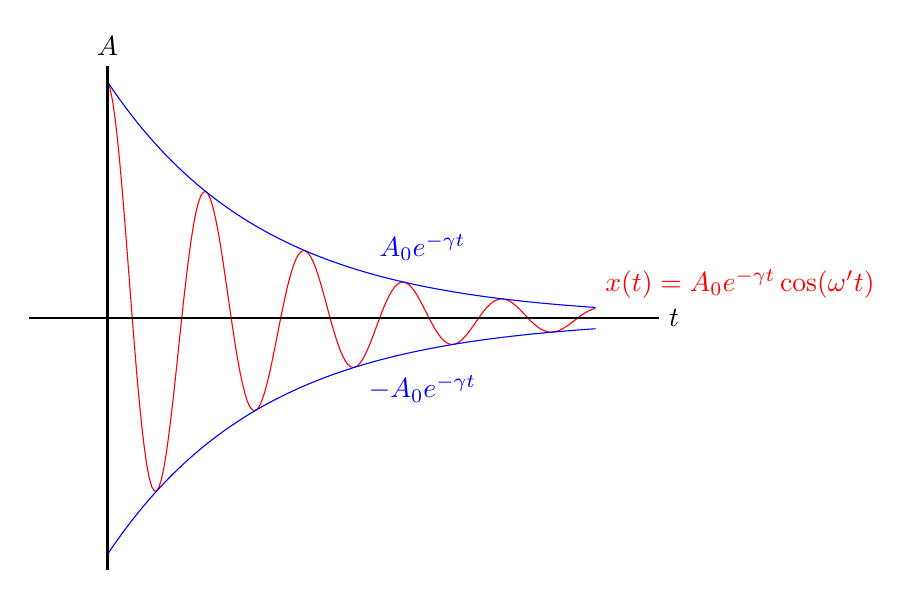
\begin{tikzpicture}[domain=0:6.2] 
						\draw [samples=200, color = red] plot
						(\x, {3*exp(-0.5*\x)*cos(5*\x r)}) node[above right] {$x(t) = A_0e^{- \gamma t} \cos (\omega' t)$};
					\draw [samples=200, color = blue] plot (\x, {3 * exp(-0.5* \x)});
					\draw[color = blue] node at (4, 0.9) {$A_0e^{-\gamma t}$};
						\draw [samples=200, color = blue] plot (\x, {-3 * exp(-0.5* \x)});
						\draw[color=blue] node at (4, -0.9) {$-A_0e^{- \gamma t}$};
						\draw[thick] (-1, 0) -- (7, 0) node[right] {$t$};
						\draw[thick] (0, -3.2) -- (0, 3.2) node[above] {$A$};
					\end{tikzpicture}
				\end{center}
			 \end{solution}
		 \item For \textit{one} of the two solutions for $\Omega$ you found in part (e), find $x(t) = \Re(z(t))$
			 in the case $\omega_0 < \gamma$. This is the overdamped oscillator. Qualitatively sketch the 
			 solution $x(t)$.

			 \begin{solution}
			 	Unlike the previous solution, here we have a case where the radical is complex-valued, so 
				we can rewrite the radical as:
				\[
				\sqrt{\omega_0^2 - \gamma^2} = \sqrt{-(\gamma^2 - \omega_0^2)} = i\sqrt{\gamma^2 - \omega_0^2}   
				\] 
				Now, we define $\omega' = \sqrt{\gamma^2- \omega_0^2}$, so we can write our solution $z(t)$ as:
				\[
					z(t) = A_0e^{i (i \gamma + i \omega') t}
				\] 
				simplifying this, we get
				\[
					z(t) = A_0e^{(- \gamma - \omega')t}
				\] 
				And since there is no complex phase any longer, we have $\Re(z(t)) = z(t)$:
				\[
					\Re(z(t)) = A_0e^{-(\gamma + \omega') t}
				\] 
				Plotting this, we get:
				\begin{center}
					\begin{tikzpicture}[domain=0:6.2]
						\draw[samples=200, color=red] plot (\x, {3*exp(-0.7*\x)}) node[above] {$x(t) = A_0e^{- (\gamma + \omega')t}$};
						\draw(-1, 0) -- (7, 0) node[right] {$t$};
						\draw(0, -3.2) -- (0, 3.2) node[above] {$A$};
					\end{tikzpicture}
				\end{center}
				there isn't really any fancy envelope I can draw for this curve so the plot looks kind of lame,
				but the lack of an oscillation is exactly what we expect for an overdamped oscillator. 
			 \end{solution}
	 \end{enumerate}
\end{document}
